\section{PackStack Configuration}
\label{app:packstack-config}

Once OpenStack PackStack is installed, the deployment can be customized
for particular use cases and to use nonstandard storage locations. In
this section the environment setup is described and the commands or
actions used to configure the environment are shown. Further this
section details how to configure OpenStack to use GPFS as a back end for
storing Glance images and for Nova compute instances.

\subsection{External Network Setup}
\label{openstack-ext}
In Appendix~\ref{app:packstack-install} the necessary changes to the
network interfaces and the options supplied to the PackStack installer
allow for an External Network to be configured as described next.

This configuration roughly follows the RDO Guide~\cite{PackStacksetup},
although the commands and options have been changed to work with the
current packages.

First an external network must be created, note this assumes an
authenticated user (i.e. source keystonerc\_admin).
\begin{lstlisting}[escapechar=&]
  openstack network create &\texttt{--}&external \
  &\texttt{--}&provider-network-type flat \
  &\texttt{--}&provider-physical-network extnet \
  external_network
\end{lstlisting}

Once the external network is made, a subnet is created with the
configuration options for all hosts that connect to the subnet.

\begin{lstlisting}[escapechar=&]
  openstack subnet create --no-dhcp \
  &\texttt{--}&allocation-pool start=10.26.10.20,end=10.26.10.200 \
  &\texttt{--}&gateway 10.26.0.1 \
  &\texttt{--}&network external_network \
  &\texttt{--}&subnet-range 10.26.10.0/24 \
  external_subnet
\end{lstlisting}

This completes the setup of the external network and now guests can
request a public IP which is allocated from the range
10.26.10.20-10.26.10.200 and grants external Internet access.

\subsection{Internal Network Setup}
\label{openstack-int}
The internal network was setup using the Horizon interface. Guest VMs
are placed on an internal LAN subnet 192.168.72.0/24 and a router
connects the internal LAN to the external network created above. By
default all communication is allowed between hosts in the internal
network and guests can access the Internet but hosts external to the
private LAN cannot access the guests. To allow outside SSH access guests
are assigned external IP addresses from the 10.26.10.0/24 subnet on the
external network as configured above. Further firewall rules are added
to the guest VMs to only allow traffic from the proxy and host machine
inbound and allows all traffic outbound. More discussion about the
security is in Section~\ref{sec:security}.

The following figures give more detail about the internal network,
router, and firewall rules setup using the Horizon interface.
Figure\ref{fig:net-list} shows the list of networks available for the
admin tenant. Both the external network made from the command line and
the internal network made with the Horizon interfaces are shown here.
Figures~\ref{fig:int-overview}, \ref{fig:int-subnets}, and
\ref{fig:int-ports} show the settings of the created internal admin
network. Figure~\ref{fig:int-subnet} shows the child subnet settings for
the internal network where the guest VMs are actually connected. Next
Figures~\ref{fig:router-overview} and \ref{fig:router-if} show the
settings for the admin router used to connect and route traffic between
the internal and external networks. Figure~\ref{fig:fw} shows the rules
used to allow traffic to and from the guest VMs, if a rule is present
then that traffic is allowed, otherwise the traffic is denied. Finally,
Figure~\ref{fig:topo} shows how each of these components are connected
with the actual IP addresses assigned to each interface, note this
figure also has two VMs which are attached to the admin subnet in the
internal network.

\begin{figure}[H]
  \centering
  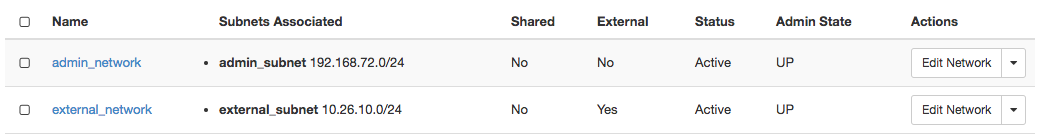
\includegraphics[scale=0.40]{img/network-netlist}
  \caption{Horizon interface listing the external network created from
the command line and the internal network made using the Horizon GUI.}
  \label{fig:net-list}
\end{figure}

\begin{figure}[H]
  \centering
  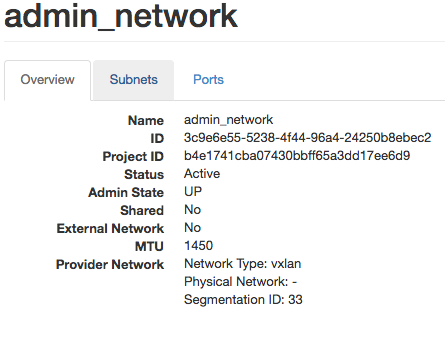
\includegraphics[scale=0.5]{img/network-adminnet-overview}
  \caption{Overview of the admin internal network settings.}
  \label{fig:int-overview}
\end{figure}

\begin{figure}[H]
  \centering
  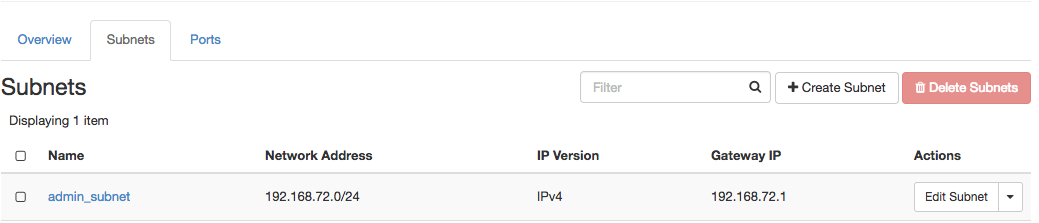
\includegraphics[scale=0.40]{img/network-adminnet-subnets}
  \caption{List of the subnets associated with the internal network.}
  \label{fig:int-subnets}
\end{figure}

\begin{figure}[H]
  \centering
  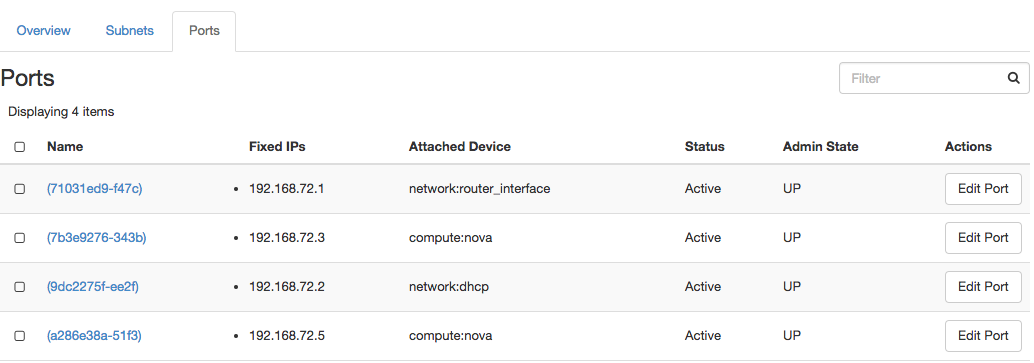
\includegraphics[scale=0.40]{img/network-adminnet-ports}
  \caption{List of ports used by the admin internal network.}
  \label{fig:int-ports}
\end{figure}

\begin{figure}[H]
  \centering
  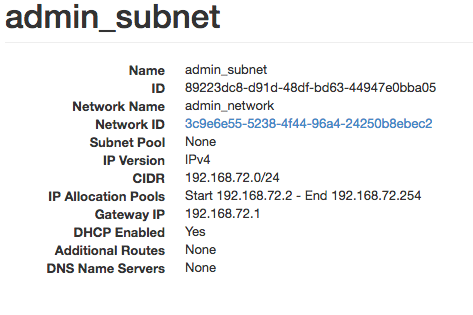
\includegraphics[scale=0.5]{img/network-adminsub-overview}
  \caption{Overview of the admin internal subnet settings.}
  \label{fig:int-subnet}
\end{figure}

\begin{figure}[H]
  \centering
  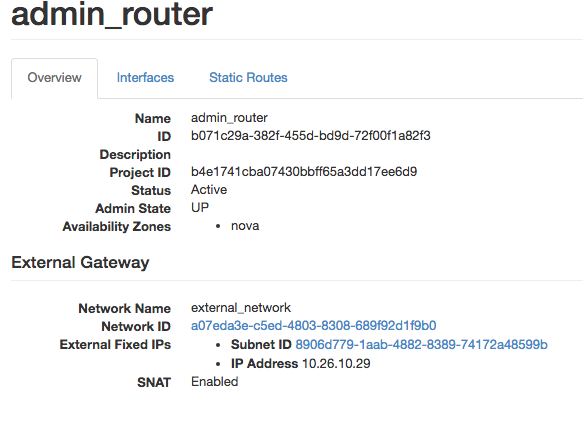
\includegraphics[scale=0.5]{img/network-adminrouter-overview}
  \caption{Overview of the admin router settings connecting the internal
and external networks.}
  \label{fig:router-overview}
\end{figure}

\begin{figure}[H]
  \centering
  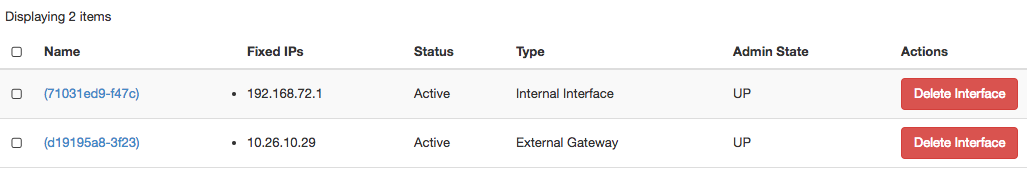
\includegraphics[scale=0.40]{img/network-adminrouter-if}
  \caption{List of interfaces on the admin router.}
  \label{fig:router-if}
\end{figure}

\begin{figure}[H]
  \centering
  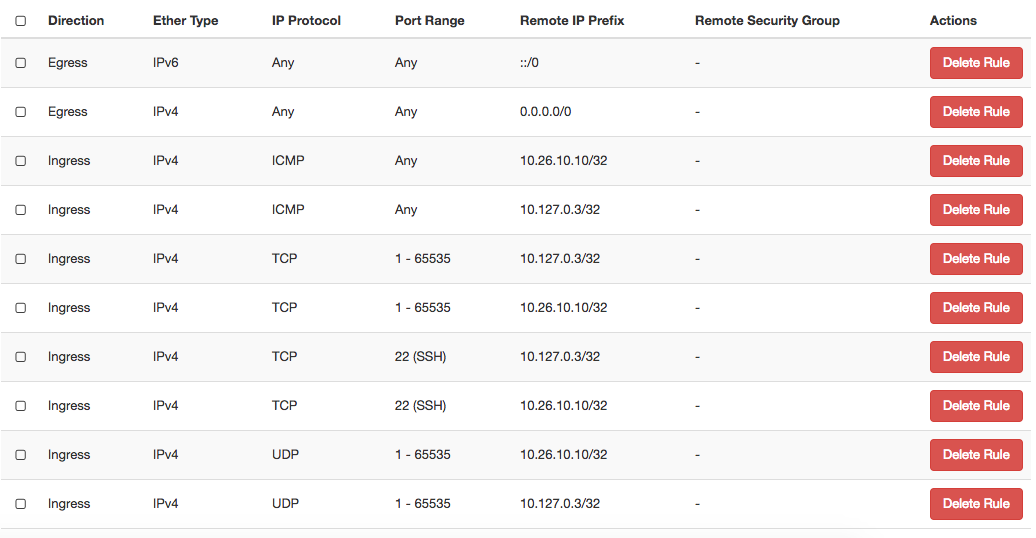
\includegraphics[scale=0.40]{img/network-fw}
  \caption{List of the firewall rules applied to the guest VMs in the
admin network.}
  \label{fig:fw}
\end{figure}

\begin{figure}[H]
  \centering
  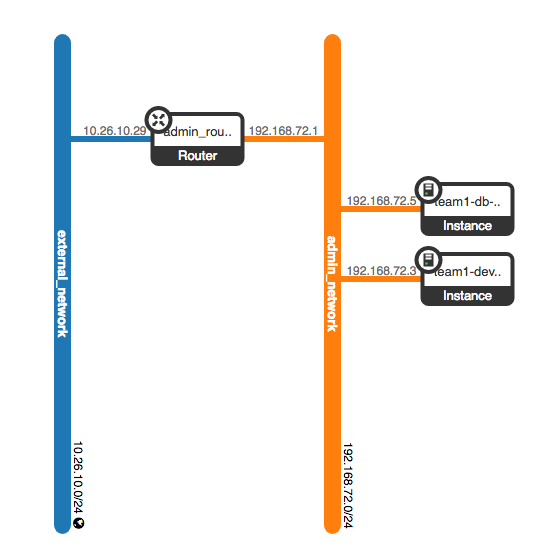
\includegraphics[scale=0.5]{img/network-topo}
  \caption{Visualization of the internal and external networks and how
the VMs are connected to each other and the Internet.}
  \label{fig:topo}
\end{figure}


\subsection{GPFS Mounting}
\label{gpfs-config}
The host machine is attached to a 144 TB IBM GPFS which can be used for
storage of images and instance backends. Before configuring the
services, ensure the GPFS was mounted in the following way.

\begin{lstlisting}[escapechar=&]
  mmstartup
  mmgetstate
  # After the GPFS system is active continue with the following
  mmmount gpfs1
  mount&\texttt{--}&bind \gpfs1/csc1 /gpfs
\end{lstlisting}
 
This mounts the GPFS at /gpfs. Following the IBM OpenStack configuration
guide~\cite{GPFSsetup}, inside the gpfs directory create the following 
directories. 

\begin{lstlisting}[escapechar=&]
  cd /gpfs
  mkdir OpenStack
  mkdir OpenStack/glance
  mkdir OpenStack/glance/images
  mkdir OpenStack/nova
  mkdir OpenStack/nova/instance
  chown -R glance:glance OpenStack/glance
  chown -R nova:nova OpenStack/nova
\end{lstlisting}

\subsubsection{Glance GPFS Configuration}

In /etc/glance/glance-api.conf edit the following three lines.

\begin{lstlisting}[escapechar=&]
  show_multiple_locations = True
  filesystem_store_default_datadir = /gpfs/OpenStack/glance/images
  filesystem_store_metadata_file = /etc/glance/glance-images.json
\end{lstlisting}

Next, from the command line run uuidgen to get an id.

\begin{lstlisting}[escapechar=&]
  $ uuidgen
  d80f3398-41bd-465c-8356-335959dea05d
\end{lstlisting}

Then open /etc/glance/glance-images.json and make the following changes.
\begin{lstlisting}[escapechar=&]
{
  "id": "d80f3398-41bd-465c-8356-335959dea05d",
  "mountpoint": "/gpfs"
}
\end{lstlisting}

Finally restart the glance services.
\begin{lstlisting}[escapechar=&]
  sudo service openstack-glance-api restart
  sudo service openstack-glance-registry restart
\end{lstlisting}

\subsubsection{Nova GPFS Configuration}

In the /etc/nova/nova.conf file make the following changes.
\begin{lstlisting}[escapechar=&]
  instance_path=/gpfs/OpenStack/nova/instances
  disk_cachemodes=file=writeback
  allowed_direct_url_schemes=file
  [image_file_url]
  filesystems=gpfs
  [image_file_url:gpfs]
  id="d80f3398-41bd-465c-8356-335959dea05d"
\end{lstlisting}

Note the last two lines must be added manually and the id is the same as
the one generated above.

Once the changes are made restart the nova services.

\begin{lstlisting}[escapechar=&]
  sudo service openstack-nova-compute restart
  sudo service openstack-nova-api restart
  sudo service openstack-nova-scheduler restart
  sudo service openstack-nova-conductor restart
  sudo service openstack-nova-cert restart
\end{lstlisting}
